%  LaTeX support: latex@mdpi.com
%  In case you need support, please attach all files that are necessary for compiling as well as the log file, and specify the details of your LaTeX setup (which operating system and LaTeX version / tools you are using).

%=================================================================
\documentclass[tropicalmed,article,submit,moreauthors,pdftex]{mdpi}

% If you would like to post an early version of this manuscript as a preprint, you may use preprint as the journal and change 'submit' to 'accept'. The document class line would be, e.g., \documentclass[preprints,article,accept,moreauthors,pdftex]{mdpi}. This is especially recommended for submission to arXiv, where line numbers should be removed before posting. For preprints.org, the editorial staff will make this change immediately prior to posting.

%% Some pieces required from the pandoc template
\providecommand{\tightlist}{%
  \setlength{\itemsep}{0pt}\setlength{\parskip}{4pt}}
\setlist[itemize]{leftmargin=*,labelsep=5.8mm}
\setlist[enumerate]{leftmargin=*,labelsep=4.9mm}

\usepackage{longtable}

% see https://stackoverflow.com/a/47122900

%--------------------
% Class Options:
%--------------------
%----------
% journal
%----------
% Choose between the following MDPI journals:
% acoustics, actuators, addictions, admsci, aerospace, agriculture, agriengineering, agronomy, algorithms, animals, antibiotics, antibodies, antioxidants, applsci, arts, asc, asi, atmosphere, atoms, axioms, batteries, bdcc, behavsci , beverages, bioengineering, biology, biomedicines, biomimetics, biomolecules, biosensors, brainsci , buildings, cancers, carbon , catalysts, cells, ceramics, challenges, chemengineering, chemistry, chemosensors, children, cleantechnol, climate, clockssleep, cmd, coatings, colloids, computation, computers, condensedmatter, cosmetics, cryptography, crystals, dairy, data, dentistry, designs , diagnostics, diseases, diversity, drones, econometrics, economies, education, electrochem, electronics, energies, entropy, environments, epigenomes, est, fermentation, fibers, fire, fishes, fluids, foods, forecasting, forests, fractalfract, futureinternet, futurephys, galaxies, games, gastrointestdisord, gels, genealogy, genes, geohazards, geosciences, geriatrics, hazardousmatters, healthcare, heritage, highthroughput, horticulturae, humanities, hydrology, ijerph, ijfs, ijgi, ijms, ijns, ijtpp, informatics, information, infrastructures, inorganics, insects, instruments, inventions, iot, j, jcdd, jcm, jcp, jcs, jdb, jfb, jfmk, jimaging, jintelligence, jlpea, jmmp, jmse, jnt, jof, joitmc, jpm, jrfm, jsan, land, languages, laws, life, literature, logistics, lubricants, machines, magnetochemistry, make, marinedrugs, materials, mathematics, mca, medicina, medicines, medsci, membranes, metabolites, metals, microarrays, micromachines, microorganisms, minerals, modelling, molbank, molecules, mps, mti, nanomaterials, ncrna, neuroglia, nitrogen, notspecified, nutrients, ohbm, particles, pathogens, pharmaceuticals, pharmaceutics, pharmacy, philosophies, photonics, physics, plants, plasma, polymers, polysaccharides, preprints , proceedings, processes, proteomes, psych, publications, quantumrep, quaternary, qubs, reactions, recycling, religions, remotesensing, reports, resources, risks, robotics, safety, sci, scipharm, sensors, separations, sexes, signals, sinusitis, smartcities, sna, societies, socsci, soilsystems, sports, standards, stats, surfaces, surgeries, sustainability, symmetry, systems, technologies, test, toxics, toxins, tropicalmed, universe, urbansci, vaccines, vehicles, vetsci, vibration, viruses, vision, water, wem, wevj

%---------
% article
%---------
% The default type of manuscript is "article", but can be replaced by:
% abstract, addendum, article, benchmark, book, bookreview, briefreport, casereport, changes, comment, commentary, communication, conceptpaper, conferenceproceedings, correction, conferencereport, expressionofconcern, extendedabstract, meetingreport, creative, datadescriptor, discussion, editorial, essay, erratum, hypothesis, interestingimages, letter, meetingreport, newbookreceived, obituary, opinion, projectreport, reply, retraction, review, perspective, protocol, shortnote, supfile, technicalnote, viewpoint
% supfile = supplementary materials

%----------
% submit
%----------
% The class option "submit" will be changed to "accept" by the Editorial Office when the paper is accepted. This will only make changes to the frontpage (e.g., the logo of the journal will get visible), the headings, and the copyright information. Also, line numbering will be removed. Journal info and pagination for accepted papers will also be assigned by the Editorial Office.

%------------------
% moreauthors
%------------------
% If there is only one author the class option oneauthor should be used. Otherwise use the class option moreauthors.

%---------
% pdftex
%---------
% The option pdftex is for use with pdfLaTeX. If eps figures are used, remove the option pdftex and use LaTeX and dvi2pdf.

%=================================================================
\firstpage{1}
\makeatletter
\setcounter{page}{\@firstpage}
\makeatother
\pubvolume{xx}
\issuenum{1}
\articlenumber{5}
\pubyear{2019}
\copyrightyear{2019}
%\externaleditor{Academic Editor: name}
\history{Received: date; Accepted: date; Published: date}
\updates{yes} % If there is an update available, un-comment this line

%% MDPI internal command: uncomment if new journal that already uses continuous page numbers
%\continuouspages{yes}

%------------------------------------------------------------------
% The following line should be uncommented if the LaTeX file is uploaded to arXiv.org
%\pdfoutput=1

%=================================================================
% Add packages and commands here. The following packages are loaded in our class file: fontenc, calc, indentfirst, fancyhdr, graphicx, lastpage, ifthen, lineno, float, amsmath, setspace, enumitem, mathpazo, booktabs, titlesec, etoolbox, amsthm, hyphenat, natbib, hyperref, footmisc, geometry, caption, url, mdframed, tabto, soul, multirow, microtype, tikz

%=================================================================
%% Please use the following mathematics environments: Theorem, Lemma, Corollary, Proposition, Characterization, Property, Problem, Example, ExamplesandDefinitions, Hypothesis, Remark, Definition
%% For proofs, please use the proof environment (the amsthm package is loaded by the MDPI class).

%=================================================================
% Full title of the paper (Capitalized)
\Title{Lessons learned and paths forward for rabies dog vaccination in
Madagascar: a case study of pilot vaccination campaigns in Moramanga
District}

% Authors, for the paper (add full first names)
\Author{Caitlynn Filla$^{1, \dagger}$, Malavika Rajeev$^{2,
\dagger}$\href{https://orcid.org/0000-0001-6030-4995}{\orcidicon}, Zoavina
Randriana$^{3}$, Chantal Hanitriniana$^{4}$, Radoniaina R.
Rafaliarison$^{3}$, Glenn Edosoa$^{5}$, Mamitiana
Andriamananjara$^{6}$, Nivohanitra P. Razafindraibe$^{6}$, José
Nely$^{7}$, Angelique Ferreira$^{3, 8}$, Annie Yang$^{2,
\ddagger}$, Fenomanana Daniel$^{3}$, Tara A. Clarke$^{3, 9}$, Zachary
Farris$^{3, 10}$, Terry Stone$^{8}$, Jochem Lastdrager$^{8}$, Tsiky
Rajaonarivelo$^{3}$, Katie Hampson$^{11}$, C. Jessica E.
Metcalf$^{2}$, Kim Valenta$^{1, 3}$}

% Authors, for metadata in PDF
\AuthorNames{Caitlynn Filla, Malavika Rajeev, Zoavina Randriana, Chantal
Hanitriniana, Radoniaina R. Rafaliarison, Glenn Edosoa, Mamitiana
Andriamananjara, Nivohanitra P. Razafindraibe, José Nely, Angelique
Ferreira, Annie Yang, Fenomanana Daniel, Tara A. Clarke, Zachary
Farris, Terry Stone, Jochem Lastdrager, Tsiky Rajaonarivelo, Katie
Hampson, C. Jessica E. Metcalf, Kim Valenta}

% Affiliations / Addresses (Add [1] after \address if there is only one affiliation.)
\address{%
$^{1}$ \quad University of Florida, Department of Anthropology
Gainesville, Florida, USA; \\
$^{2}$ \quad Department of Ecology and Evolutionary Biology, Princeton
University Princeton, NJ, United States; \\
$^{3}$ \quad The Mad Dog Initiative Akanin'ny Veterinera, Akaikiniarivo,
Ambatobe, Antananarivo 101, Madagascar; \\
$^{4}$ \quad Mention Zoologie et Biodiversité Animale, Faculté des
Sciences Université d'Antananarivo, Antananarivo, Madagascar; \\
$^{5}$ \quad Chargé des Maladies Tropicales Négligées Organisation
mondiale de la Santé Madagascar, Antananarivo, Madagascar; \\
$^{6}$ \quad Direction des Services Vétérinaires Ministère chargé de
l'Agriculture et de l'Élevage, Antananarivo, Madagascar; \\
$^{7}$ \quad Service contre les Maladies Endémo-épidémiques et
Tropicales Négligées Ministère de la Santé Publique, Antananarivo,
Madagascar; \\
$^{8}$ \quad Travelling Animal Doctors 919 Crossan Rd, Newark, Delaware,
USA; \\
$^{9}$ \quad North Carolina State University, Department of Sociology
and Anthropology Raleigh, North Carolina, USA; \\
$^{10}$ \quad Appalachian State University, Department of Health and
Exercise Science Boone, North Carolina, USA; \\
$^{11}$ \quad Boyd Orr Centre for Population and Ecosystem Health
Institute of Biodiversity, Animal Health and Comparative Medicine
University of Glasgow, Glasgow, UK; \\
}
% Contact information of the corresponding author
\corres{Correspondence: \href{mailto:mrajeev@princeton.edu}{\nolinkurl{mrajeev@princeton.edu}}}

% Current address and/or shared authorship
\firstnote{These authors contributed equally to this work.}
\secondnote{Deceased.}






% The commands \thirdnote{} till \eighthnote{} are available for further notes

% Simple summary

% Abstract (Do not insert blank lines, i.e. \\)
\abstract{Canine rabies causes an estimated 60,000 human deaths per
year, but these deaths are preventable through post-exposure prophylaxis
of people and vaccination of domestic dogs. Dog vaccination campaigns
targeting 70\% of the population are effective at interrupting
transmission. Here, we report on lessons learned during pilot dog
vaccination campaigns in the Moramanga District of Madagascar. We
compare two different vaccination strategies: a volunteer driven effort
to vaccinate dogs in two communes using static point vaccination, and
continuous vaccination as part of routine veterinary services. We used
dog age data from the campaigns to estimate key demographic parameters
and to simulate different vaccination strategies. Overall, we found that
dog vaccination was feasible and that most dogs were accessible to
vaccination. The static-point campaign achieved higher coverage, but
required more resources and had a limited geographic scope compared to
the continuous delivery campaign. Our modeling results suggest that
targeting puppies through community-based vaccination efforts could
improve coverage. We found that mass dog vaccination is feasible and can
achieve high coverage in Madagascar, however context-specific strategies
and an investment in dog vaccination as a public good will be required
to move the country towards elimination.}

% Keywords
\keyword{canine rabies; mass dog vaccination; central point vaccination;
puppy vaccination; Zeroby30;}

% The fields PACS, MSC, and JEL may be left empty or commented out if not applicable
%\PACS{J0101}
%\MSC{}
%\JEL{}

%%%%%%%%%%%%%%%%%%%%%%%%%%%%%%%%%%%%%%%%%%
% Only for the journal Diversity
%\LSID{\url{http://}}

%%%%%%%%%%%%%%%%%%%%%%%%%%%%%%%%%%%%%%%%%%
% Only for the journal Applied Sciences:
%\featuredapplication{Authors are encouraged to provide a concise description of the specific application or a potential application of the work. This section is not mandatory.}
%%%%%%%%%%%%%%%%%%%%%%%%%%%%%%%%%%%%%%%%%%

%%%%%%%%%%%%%%%%%%%%%%%%%%%%%%%%%%%%%%%%%%
% Only for the journal Data:
%\dataset{DOI number or link to the deposited data set in cases where the data set is published or set to be published separately. If the data set is submitted and will be published as a supplement to this paper in the journal Data, this field will be filled by the editors of the journal. In this case, please make sure to submit the data set as a supplement when entering your manuscript into our manuscript editorial system.}

%\datasetlicense{license under which the data set is made available (CC0, CC-BY, CC-BY-SA, CC-BY-NC, etc.)}

%%%%%%%%%%%%%%%%%%%%%%%%%%%%%%%%%%%%%%%%%%
% Only for the journal Toxins
%\keycontribution{The breakthroughs or highlights of the manuscript. Authors can write one or two sentences to describe the most important part of the paper.}

%\setcounter{secnumdepth}{4}
%%%%%%%%%%%%%%%%%%%%%%%%%%%%%%%%%%%%%%%%%%

% Pandoc citation processing

\usepackage{amsmath}
\usepackage{booktabs}
\usepackage{caption}
\usepackage{longtable}

\begin{document}
%%%%%%%%%%%%%%%%%%%%%%%%%%%%%%%%%%%%%%%%%%

\hypertarget{introduction}{%
\section{Introduction}\label{introduction}}

Canine rabies results in an estimated 60,000 human deaths per year
globally \citep{hampson2015}. These deaths are entirely preventable:
prompt post-exposure prophylaxis of humans exposed to rabies is highly
effective at preventing death and mass dog vaccination can interrupt
transmission in domestic dogs and eventually lead to disease elimination
\citep{fooks2014}. The World Health Organization (WHO) and its partners
have set a goal to eliminate human deaths due to canine rabies by the
year 2030 (`ZeroBy30')\citep{abela-ridder2016}. Annual dog vaccination
campaigns achieving at least 70\% coverage are the recommended target
for controlling rabies in domestic dog populations
\citep{worldhealthorganization2013}. However, achieving this coverage
target in low and middle income countries where the burden of human
rabies is highest can be challenging due to economic, ecological,
sociocultural, and political barriers \citep{fahrion2017}.

In sub-Saharan African countries, parenteral vaccinations implemented
through static point campaigns have been shown to be cost-effective and
feasible \citep{borse2018}. While most dogs in these settings are
considered free roaming, they are mostly owned and are accessible for
vaccination through these campaigns \citep{morters2014, jibat2015}.
However, reaching high coverage and maintaining vaccination campaigns at
scale requires sustained investment and coordination, and the challenges
in implementation largely reflect financial and logistical constraints
more than the feasibility of vaccination itself \citep{fahrion2017}.
Developing clear and context-specific strategies and lowering costs and
resources needed could help spur the implementation and scaling up of
campaigns in these countries.

In Madagascar, canine rabies has been endemic for over a century, and
for most of that period, the Institut Pasteur de Madagascar has provided
post-exposure prophylaxis free-of-charge to bite patients in the country
\citep{reynes2011}. Currently, there are only 31 clinics where these
human vaccines are available, and there is minimal dog vaccination due
to high costs to owners and lack of vaccine availability
\citep{rajeev2018}. Recent studies have estimated a high burden of human
deaths, masked by weak surveillance across the country
\citep{rajeev2020, rajeev2018}.

The veterinary sector is largely private, with 204 veterinarians
employed in hybrid private/public employment as designated district
veterinarians. While dog vaccination is rare, livestock officers and
veterinarians work together to implement cattle vaccination campaigns
for anthrax on an annual basis as mandated by the government (owners are
charged a fee per animal for these vaccines which vary by location)
\citep{mondiale2017evaluation}. No routine mass dog vaccinations have
been conducted on the island, although a few pilot programs have begun
in recent years, largely implemented by NGO-government partnerships.

Here, we summarize lessons learned through the implementation of pilot
vaccination programs in the Moramanga District of Madagascar, where
previous work has shown high incidence of dog rabies cases and human
rabies exposures. In 2018 and 2019, we deployed two different
vaccination strategies. In 2018, we carried out a larger scale
volunteer-led pilot vaccination campaign in two communes (sub-district
level) using a static point strategy. In 2019/2020, we provided
vaccines, all necessary supplies for vaccine administration, and a
per-vaccine fee to the District Veterinarian to vaccinate animals as
part of routine services delivered continuously. We compare time, human
resources, costs, and coverage estimates between these campaigns, and
using a demographic and vaccination model we further explore different
vaccination strategies based on what we learned during implementation.

\hypertarget{methods}{%
\section{Methods}\label{methods}}

\hypertarget{study-area}{%
\subsection{Study Area}\label{study-area}}

The Moramanga District is located midway between the central highlands
and the east coast of Madagascar, at an average altitude of 936 m. It
comprises 21 communes, covering approximately 7150 km\textsuperscript{2}
with an approximate human population of 347,000\citep{instat2021}.
Previous work in the district has established a high burden of rabies
exposures and deaths despite the availability of post-exposure
prophylaxis at the district hospital \citep{rajeev2018}. While Moramanga
is relatively close to the capital city of Antananarivo
(\textasciitilde{} 3 hours by bus), within the district, travel times
between locations are highly variable, with much of the population
living in more rural areas with limited access to roads and
transportation \citep{rajeev2020}. Before 2018, there were limited
animal rabies vaccination services, with most animal vaccines available
in the urban commune of Moramanga Ville where owners were often charged
\textgreater{} 15,000 Ariary (\textasciitilde{} 4.28 USD) per vaccine
administered.

\hypertarget{campaign}{%
\subsection{2018 Campaign}\label{campaign}}

In 2018, two NGOs (the Mad Dog Initiative (MDI) and Traveling Animal
Doctors (TAD)) organized a pilot vaccination campaign in collaboration
with the Department of Veterinary Services, and the Ministry of Public
Health in the District of Moramanga. This campaign focused on two
communes in Moramanga, Moramanga Ville (the district center) and
Andasibe (a rural commune surrounding Andasibe National Park), where
previously high incidence of probable rabies exposures (Moramanga Ville)
and a high burden of deaths (Andasibe) had been recorded
\citep{rajeev2018}.

The campaign was planned as a series of static point vaccination
stations covering 1 - 3 fokontany (i.e., sub-communes) per day. A week
before the campaign dates, the vaccination team informed the chief of
the fokontany about the campaign and provided posters advertising the
date of the vaccine and that it would be available at no cost to owners.
During the campaign, we used Rabisin (10 mL vials with 1 mL per dose,
Boehringer Ingelheim) to vaccinate both dogs and cats presented that
were at least 1 month old. As part of the campaign, owners were surveyed
by vaccinators about how many dogs and cats they owned in total (split
by \textgreater{} 1 year vs.~\textless{} 1 year in order to avoid
language ambiguities that might result in excluding puppies and
kittens), as well as if their dogs were free roaming (no restrictions on
movement by the owner/`mirenyreny', tied/`mifatora', or
fenced/`mifefy'). Vaccinations were delivered at no cost to owners, but
as animal vaccination is generally thought of as a paid service in
Madagascar, owners were asked how much in Ariary they would be willing
to pay to have one animal vaccinated against rabies. For each animal
vaccinated, we recorded the species (cat or dog), sex, approximate age
in years, and whether the animal had been previously vaccinated.

To assess coverage, post-vaccination coverage surveys were conducted
according to previously established
methodology\citep{sambo2017, gibson2015}. All animals vaccinated were
concurrently marked with a colored, non-toxic, livestock crayon along
the top of the head or back. Between 4 - 6 PM when dogs are most active
\citep{sambo2017} and on the same day as the campaign, in each
vaccination location two transect surveys were done. Each team (two
people per team) walked a transect for 1 hour starting in opposite
directions and accompanied by a local guide to ensure that walking paths
did not overlap. Teams recorded any marked and unmarked dogs observed,
their roaming status (whether roaming, inside a fence, or tied), and
their approximate age (greater or less than 1 year of age).

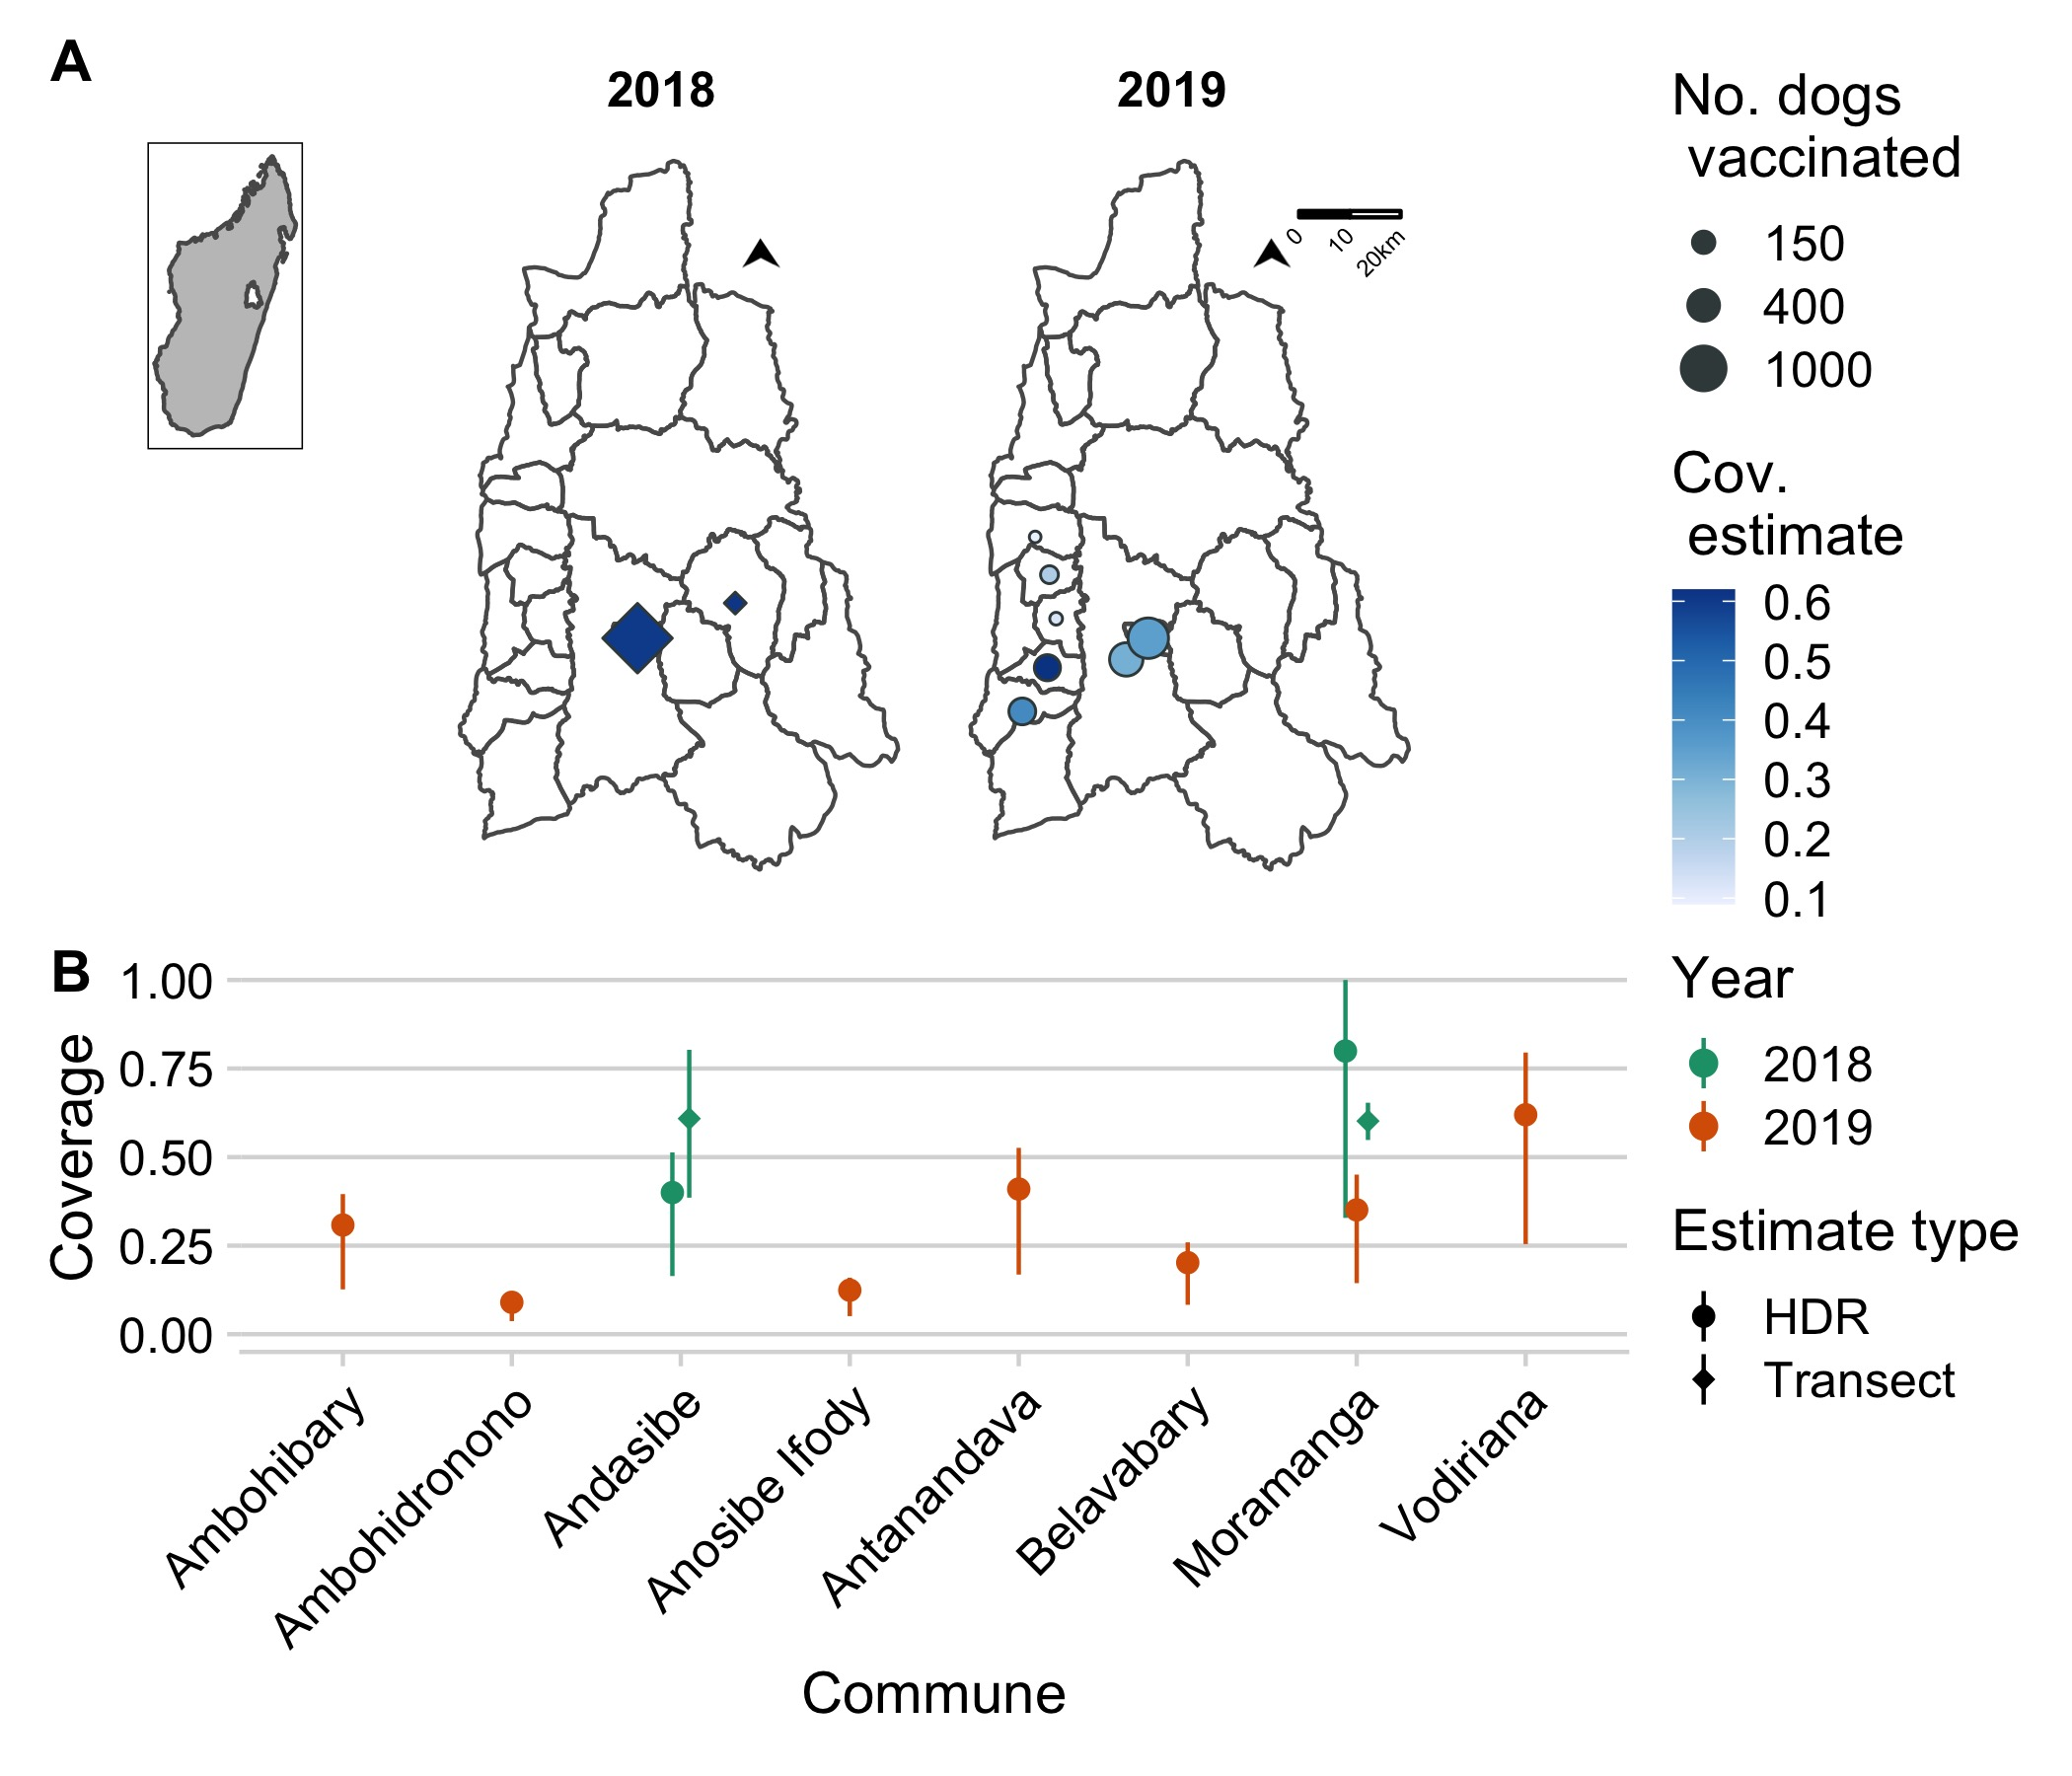
\includegraphics[width=0.8\linewidth]{/Users/mrajeev/Documents/Projects/mora_vax/figs/fig1}

\hypertarget{figure-1.-photos-from-the-2018-campaign.-topleft-advertisement-for-the-campaign-posted-on-the-door-of-the-fokontany-office-as-the-campaign-starts-topright-a-dog-post-vaccination-marked-with-a-crayon-bottomleft-a-basket-of-puppies-brought-for-vaccination-bottomright-a-line-of-owners-and-dogs-waiting-for-vaccination.}{%
\paragraph{\texorpdfstring{\textbf{Figure 1. Photos from the 2018
campaign}. \emph{Topleft: advertisement for the campaign posted on the
door of the fokontany office as the campaign starts; Topright: a dog
post-vaccination marked with a crayon; Bottomleft: a basket of puppies
brought for vaccination; Bottomright: a line of owners and dogs waiting
for
vaccination.}}{Figure 1. Photos from the 2018 campaign. Topleft: advertisement for the campaign posted on the door of the fokontany office as the campaign starts; Topright: a dog post-vaccination marked with a crayon; Bottomleft: a basket of puppies brought for vaccination; Bottomright: a line of owners and dogs waiting for vaccination.}}\label{figure-1.-photos-from-the-2018-campaign.-topleft-advertisement-for-the-campaign-posted-on-the-door-of-the-fokontany-office-as-the-campaign-starts-topright-a-dog-post-vaccination-marked-with-a-crayon-bottomleft-a-basket-of-puppies-brought-for-vaccination-bottomright-a-line-of-owners-and-dogs-waiting-for-vaccination.}}

\hypertarget{campaign-1}{%
\subsection{2019 Campaign}\label{campaign-1}}

For the 2019 campaign, instead of a static point campaign strategy,
vaccine vials(Rabisin) and the supplies needed to administer them
(needle, syringe, vaccination card for owners) were distributed to the
District Veterinarian, who then delivered the vaccination at no cost to
owners, but was directly compensated 1,500 Ar (\textasciitilde{} 0.40
USD) per rabies vaccine administered. The campaign lasted from September
6, 2019 to June 19, 2020, One week prior to her visiting each location,
the District Veterinarian advertised the vaccines by calling ahead to
the fokontany leaders and other officials who then advertised to their
communities, largely through word-of-mouth. For each animal vaccinated,
the District Veterinarian collected the animal's age and sex, and also
asked owners to approximate the distance they travelled to receive the
vaccination in meters. Researchers communicated with the District
Veterinarian about progress periodically throughout the campaign,
primarily through telephone calls. No other compensation or instructions
were provided, and we asked the District Veterinarian to administer as
many (or as few) as feasible or wanted. As the vaccinations were
delivered continuously, we were unable to do comparable post-vaccination
surveys.

\hypertarget{analyses}{%
\subsection{Analyses}\label{analyses}}

\hypertarget{campaign-resource-and-cost-comparisons}{%
\subsubsection{Campaign resource and cost
comparisons}\label{campaign-resource-and-cost-comparisons}}

We documented the overall costs and resources required for the two
vaccination efforts. We tracked the number of vaccination points, the
number of days over which these vaccinations occurred, and the number of
person days required overall (i.e.~the number of working people per day
over the campaign \citep{mazeri2021}), in addition to monetary costs. As
costs were incurred in both USD and Ariary, and the exchange rate
declined rapidly between 2018 and 2019, we used the midpoint between the
two years (3314 Ar to 1 USD) for the cost comparisons.

For the 2018 campaign, we broke costs down into the following
categories: direct vaccine costs (cost for vaccine, syringes, needles,
vaccination cards), supplies (livestock crayons, muzzles, gloves,
alcohol, swabs), food and lodging for NGO personnel and other
vaccinators during the campaign, personnel costs (per diems for the
district veterinarian, livestock field officers, local guides, and NGO
employees), and advertisement (posters and banners for advertising the
campaign). Foreign NGO volunteer expenses for travel to Madagascar were
not included in these costs. Vehicles and drivers are also not included
in these costs, as the drivers' time and vehicle use were donated to the
campaign by volunteers involved in the campaign. In 2019, costs were
split into two categories, direct vaccine costs (for same items as in
2018), and personnel costs (per vaccine fee paid to the district
veterinarian), and supplies (a generator and fuel for the veterinarian
to maintain the vaccine under cold chain during power outages).
Transportation costs were also not included as the District Veterinarian
used her own vehicle and vaccinated as part of their routine veterinary
service provisioning.

We used the data on owners' reported willingness to pay for vaccines to
estimate the proportional reduction in animals vaccinated as fees are
increased. We also estimated how this would impact cost per animal
vaccinated by approximating the costs for implementation (i.e.~those
costs that remain fixed) from costs incurred per animal vaccinated
(i.e.~vaccine, syringe, vaccination card, and per vaccination fee to
District Veterinarian in 2019), and calculating the balance between the
returns from owner payments (i.e.~increases in cost recovery per animal
vaccinated) vs.~decreasing numbers of animals vaccinated overall.

\hypertarget{coverage-estimates}{%
\subsubsection{Coverage estimates}\label{coverage-estimates}}

For the 2018 campaign, we used the transect data to estimate vaccination
coverage as the proportion of dogs sighted that were marked using a
binomial confidence interval at the commune level. For the 2019
campaign, we estimated vaccination coverage using human-to-dog ratios
(HDRs) and human population estimates
\citep{cleaveland2003, athingo2020}. We used a range of 8 - 25, based on
previous data from Madagascar \citep{ratsitorahina2009} and based on
recent estimates from household surveys in the Moramanga District
\citep{leblancclaireRabiesMadagascarThreepronged2019}. We set the point
estimate using an HDR of 19.5, the midpoint between the HDRs estimated
for two communities in the District by LeBlanc et al.~2019. We used
human population estimates from the 2018 national census in each commune
where the vaccinations were delivered \citep{instat2021}. Coverage was
estimated as the number of dogs vaccinated in total in that commune
divided by the estimated dog population. We used this same method for
the 2018 campaign, as well, to compare coverage estimated by the
post-vaccination transects vs.~HDRs.

\hypertarget{dog-demography}{%
\subsubsection{Dog Demography}\label{dog-demography}}

Using the age data on vaccinated animals collected during both
vaccination campaigns, we estimated the proportion of the population in
four age classes: puppies under the age of 1 year, juveniles aged 1 - 2
yrs, adults aged 2 - 6 years, and older dogs aged 6+ years based on .
With the assumption that these estimates represent the population at a
stable age distribution, we use a Leslie matrix model to estimate annual
adult survival probability and fertility using maximum likelihood
estimation \citep{Fujiwara2017}. Specifically, we assume that the number
of individuals in each age class follows a Poisson distribution with the
mean predicted by the stable age distribution from the model (the
proportion of individuals in each age class at equilibrium, equal to the
eigenvector associated with the dominant eigenvalue of the matrix
\(\nu\)) multiplied by the total number of individuals in the population
(\(N_t\)):

\[ N_{a} \sim Pois(\nu N_t) \]

We assume that all individuals older than 1 year of age reproduce, and
we do not estimate declines in fertility given the small proportion of
dogs older than age six years in the population. To get bootstrapped
estimates, we used 100 sub-sampled data sets of 1000 observations each
from the observed age data to fit the parameters, and also varied
initial values used in the optimization (N = 100 initial values sets)
for 10,000 parameter estimates total.

\hypertarget{modeling-vaccination-campaign-strategies}{%
\subsubsection{Modeling vaccination campaign
strategies}\label{modeling-vaccination-campaign-strategies}}

We used the parameter estimates from the demographic model to simulate
different vaccination strategies in a hypothetical commune with 1000
dogs. We used a discrete time age-structured model with a monthly time
step to compare three strategies:

\begin{enumerate}
\def\labelenumi{\arabic{enumi})}
\tightlist
\item
  Annual vaccination campaigns occurring within the same month each year
  targeting dogs of all ages
\item
  Continuous vaccination of new puppies throughout the year targeting
  puppies that reach the age of 3 months
\item
  A combined approach with annual campaigns (as 1) and routine puppy
  vaccination (as 2)
\end{enumerate}

We split the dog population into puppies (\textless{} 1 year old) and
adults based on the stable age distribution estimated from the
demographic model. To estimate pup survival in year one, we took the
fertility estimates (i.e., number of new puppies per reproducing dog
observed in the pup age class) and divided by an estimate of newborn
pups per reproducing dog each year based on average litter size, average
number of litters per female per year
\citep{hampson2009, morters2014, czupryna2016}, and the proportion of
the adult population that is female (estimated from our data). We
assumed that for the annual campaign strategy, surviving vaccinated
adult dogs were revaccinated in subsequent years
\citep{delriovilas2017}, but that if a pup had been vaccinated within 9
months of the campaign, it was not revaccinated. We also assumed that
vaccine immunity lasted for a discrete period of 3 years (with
revaccination resetting immunity). A subset of parameter estimates
resulted in estimates of population decline, but based on the shape of
the age pyramid and to simulate reasonable campaign scenarios, we
filtered to parameter estimates which corresponded to positive
population growth.

\hypertarget{data-and-ethics-statement}{%
\paragraph{Data and ethics statement}\label{data-and-ethics-statement}}

All data were analysed in R version 4.0.2 (2020-06-22) \citep{R2020},
largely using the \texttt{tidyverse} package suite \citep{wickham2019}.
Geospatial data were mapped using the sf \citep{sf} package. All data
and code are available at \url{https://github.com/mrajeev08/mora_vax}.
The vaccinations were part of a public health campaign and routine
veterinary service provisioning carried out by the local veterinary
officials, the NGOs involved, and in partnership with the Ministry of
Public Health and the Department of Veterinary Services at the national
level. MDI also maintains national research permits (MICET permit:
\#130-19/MEDD/SG/DGEF/DGRNE) for its research and volunteer programs.

\hypertarget{results}{%
\section{Results}\label{results}}

\hypertarget{summary-of-2018-and-2019-campaigns}{%
\subsection{Summary of 2018 and 2019
campaigns}\label{summary-of-2018-and-2019-campaigns}}

During the 2018 campaign, a total of 3137 animals were vaccinated (2057
dogs and 1080 cats) in the Moramanga (urban) and Andasibe (rural)
communes over 13 days during the month of April (Table 1). We vaccinated
at 7 points in Andasibe and 14 points in Moramanga Ville. During the
2019 campaign, between September 2019 - June 2020, the District
Veterinarian vaccinated a total of 2385animals (1898 dogs and 486 cats)
over 48 days in seven communes in the Moramanga District. While more
animals were vaccinated per vaccination point and per vaccination day in
2018 compared to 2019, the number of animals vaccinated per person-day
was much higher for the 2019 campaign. More animals were vaccinated in
2018 vs.~2019, but this was largely a result of vaccinating more cats
during the 2018 campaign (Table 1).

In 2018, 15\% of dogs had a previous history of vaccination (largely in
the urban commune of Moramanga Ville) with only 7\% of dogs vaccinated
within the last year. This remained largely the same in 2019
(\textasciitilde{} 13\%), as the District Veterinarian focused their
efforts in other communes. The District Veterinarian did vaccinate 771
dogs in Moramanga Ville in 2019, and of those 24.9\% had been vaccinated
in the previous year's campaign, whereas only 4.9\% of dogs vaccinated
in all other communes had any history of previous vaccination. In
addition, in 2019, 2.1\% of animals had been spayed or neutered,
reflecting efforts by the Mad Dog Initiative to implement free spay and
neuter clinics in the district.

In 2018, 19\% of owners reported their animals were free-roaming, but
this varied by location (Table 1). In addition, while less than 19\% of
owners in Moramanga Ville reported that their animals were free roaming,
the majority of animals observed during the transects (77\%) were
observed outside of fences and not tied, and thus the majority of
animals could be classified as semi-confined in the more urban township
of Moramanga Ville, and free-roaming in the rural setting of Andasibe
(approximately 67\% of owners reported their dogs as free-roaming, Table
1). In 2019, the District Veterinarian also asked owners to approximate
how far they travelled in meters to get their animals vaccinated, and
94\% of people reportedly travelled less than 1 km to reach the
vaccination point.

\hypertarget{table-1.-summary-of-2018-and-2019-campaigns.-breakdown-of-of-animals-vaccinated-prior-vaccination-history-dog-demography-dog-ownership-daily-and-per-vaccination-rates-by-year-and-location-for-2018.-photo-credict-jochem-lastdrager-traveling-animal-doctors.}{%
\paragraph{\texorpdfstring{\textbf{Table 1. Summary of 2018 and 2019
campaigns}. \emph{Breakdown of of animals vaccinated, prior vaccination
history, dog demography, dog ownership, daily and per vaccination rates
by year and location (for 2018). Photo credict: Jochem Lastdrager,
Traveling Animal
Doctors.}}{Table 1. Summary of 2018 and 2019 campaigns. Breakdown of of animals vaccinated, prior vaccination history, dog demography, dog ownership, daily and per vaccination rates by year and location (for 2018). Photo credict: Jochem Lastdrager, Traveling Animal Doctors.}}\label{table-1.-summary-of-2018-and-2019-campaigns.-breakdown-of-of-animals-vaccinated-prior-vaccination-history-dog-demography-dog-ownership-daily-and-per-vaccination-rates-by-year-and-location-for-2018.-photo-credict-jochem-lastdrager-traveling-animal-doctors.}}

\captionsetup[table]{labelformat=empty,skip=1pt}
\begin{longtable}{lllll}
\toprule
& \multicolumn{3}{c}{2018} & \\ 
 \cmidrule(lr){2-4}
 & Andasibe & Moramanga Ville & All Communes & All Communes \\ 
\midrule
Total animals 
 vaccinated & 528 & 2609 & 3137 & 2385 \\ 
Total dogs 
 vaccinated & 254 & 1,803 & 2,057 & 1,898 \\ 
Dogs with history of vaccination & 5\% & 16\% & 15\% & 13\% \\ 
Dogs vaccinated within last year & 5\% & 7\% & 7\% & 13\% \\ 
Percent male dogs & 55\% & 56\% & 56\% & 65\% \\ 
Average dogs per owner & 0.8 & 1.1 & 1.0 & NA \\ 
Percent of owners with 
 free-roaming dogs & 67\% & 19\% & 28\% & NA \\ 
Animals vaccinated per day (total days) & 88 (6) & 372.7 (7) & 241.3 (13) & 49.7 (48) \\ 
Animals vaccinated per 
 vaccination point (total points) & 75.4 (7) & 186.4 (14) & 149.4 (21) & 37.3 (64) \\ 
Animals vaccinated per 
 person day (total person days) & 11.7 (45) & 21.6 (121) & 18.9 (166) & 49.7 (48) \\ 
\bottomrule
\end{longtable}

\hypertarget{cost-comparison-and-willingness-to-pay}{%
\subsection{Cost comparison and willingness to
pay}\label{cost-comparison-and-willingness-to-pay}}

The 2018 campaign cost more overall and per animal vaccinated than the
2019 campaign, largely due to increased personnel costs (fig 2A \& B,
Table 1). Reflecting the extra personnel necessary to run the static
point campaign, the 2018 campaign also took substantially more
person-days per animal vaccinated (Table 1). We found that charging
owners for vaccination would result in minimal cost recovery (fig 2C)
and beyond a minimal cost would actually result in increased costs per
vaccinated individual than free-of-charge campaigns. Cost recovery would
be more likely given a 2019 style strategy where the majority of the
costs are incurred on a per animal basis, compared to the 2018 campaigns
where the costs are largely due to setting up the static point
vaccination stations (fig 4A). More importantly, in all cases, even a
nominal fee would significantly reduce numbers of dogs vaccinated and
thus vaccination coverage, particularly in the rural commune of Andasibe
(fig 2D).

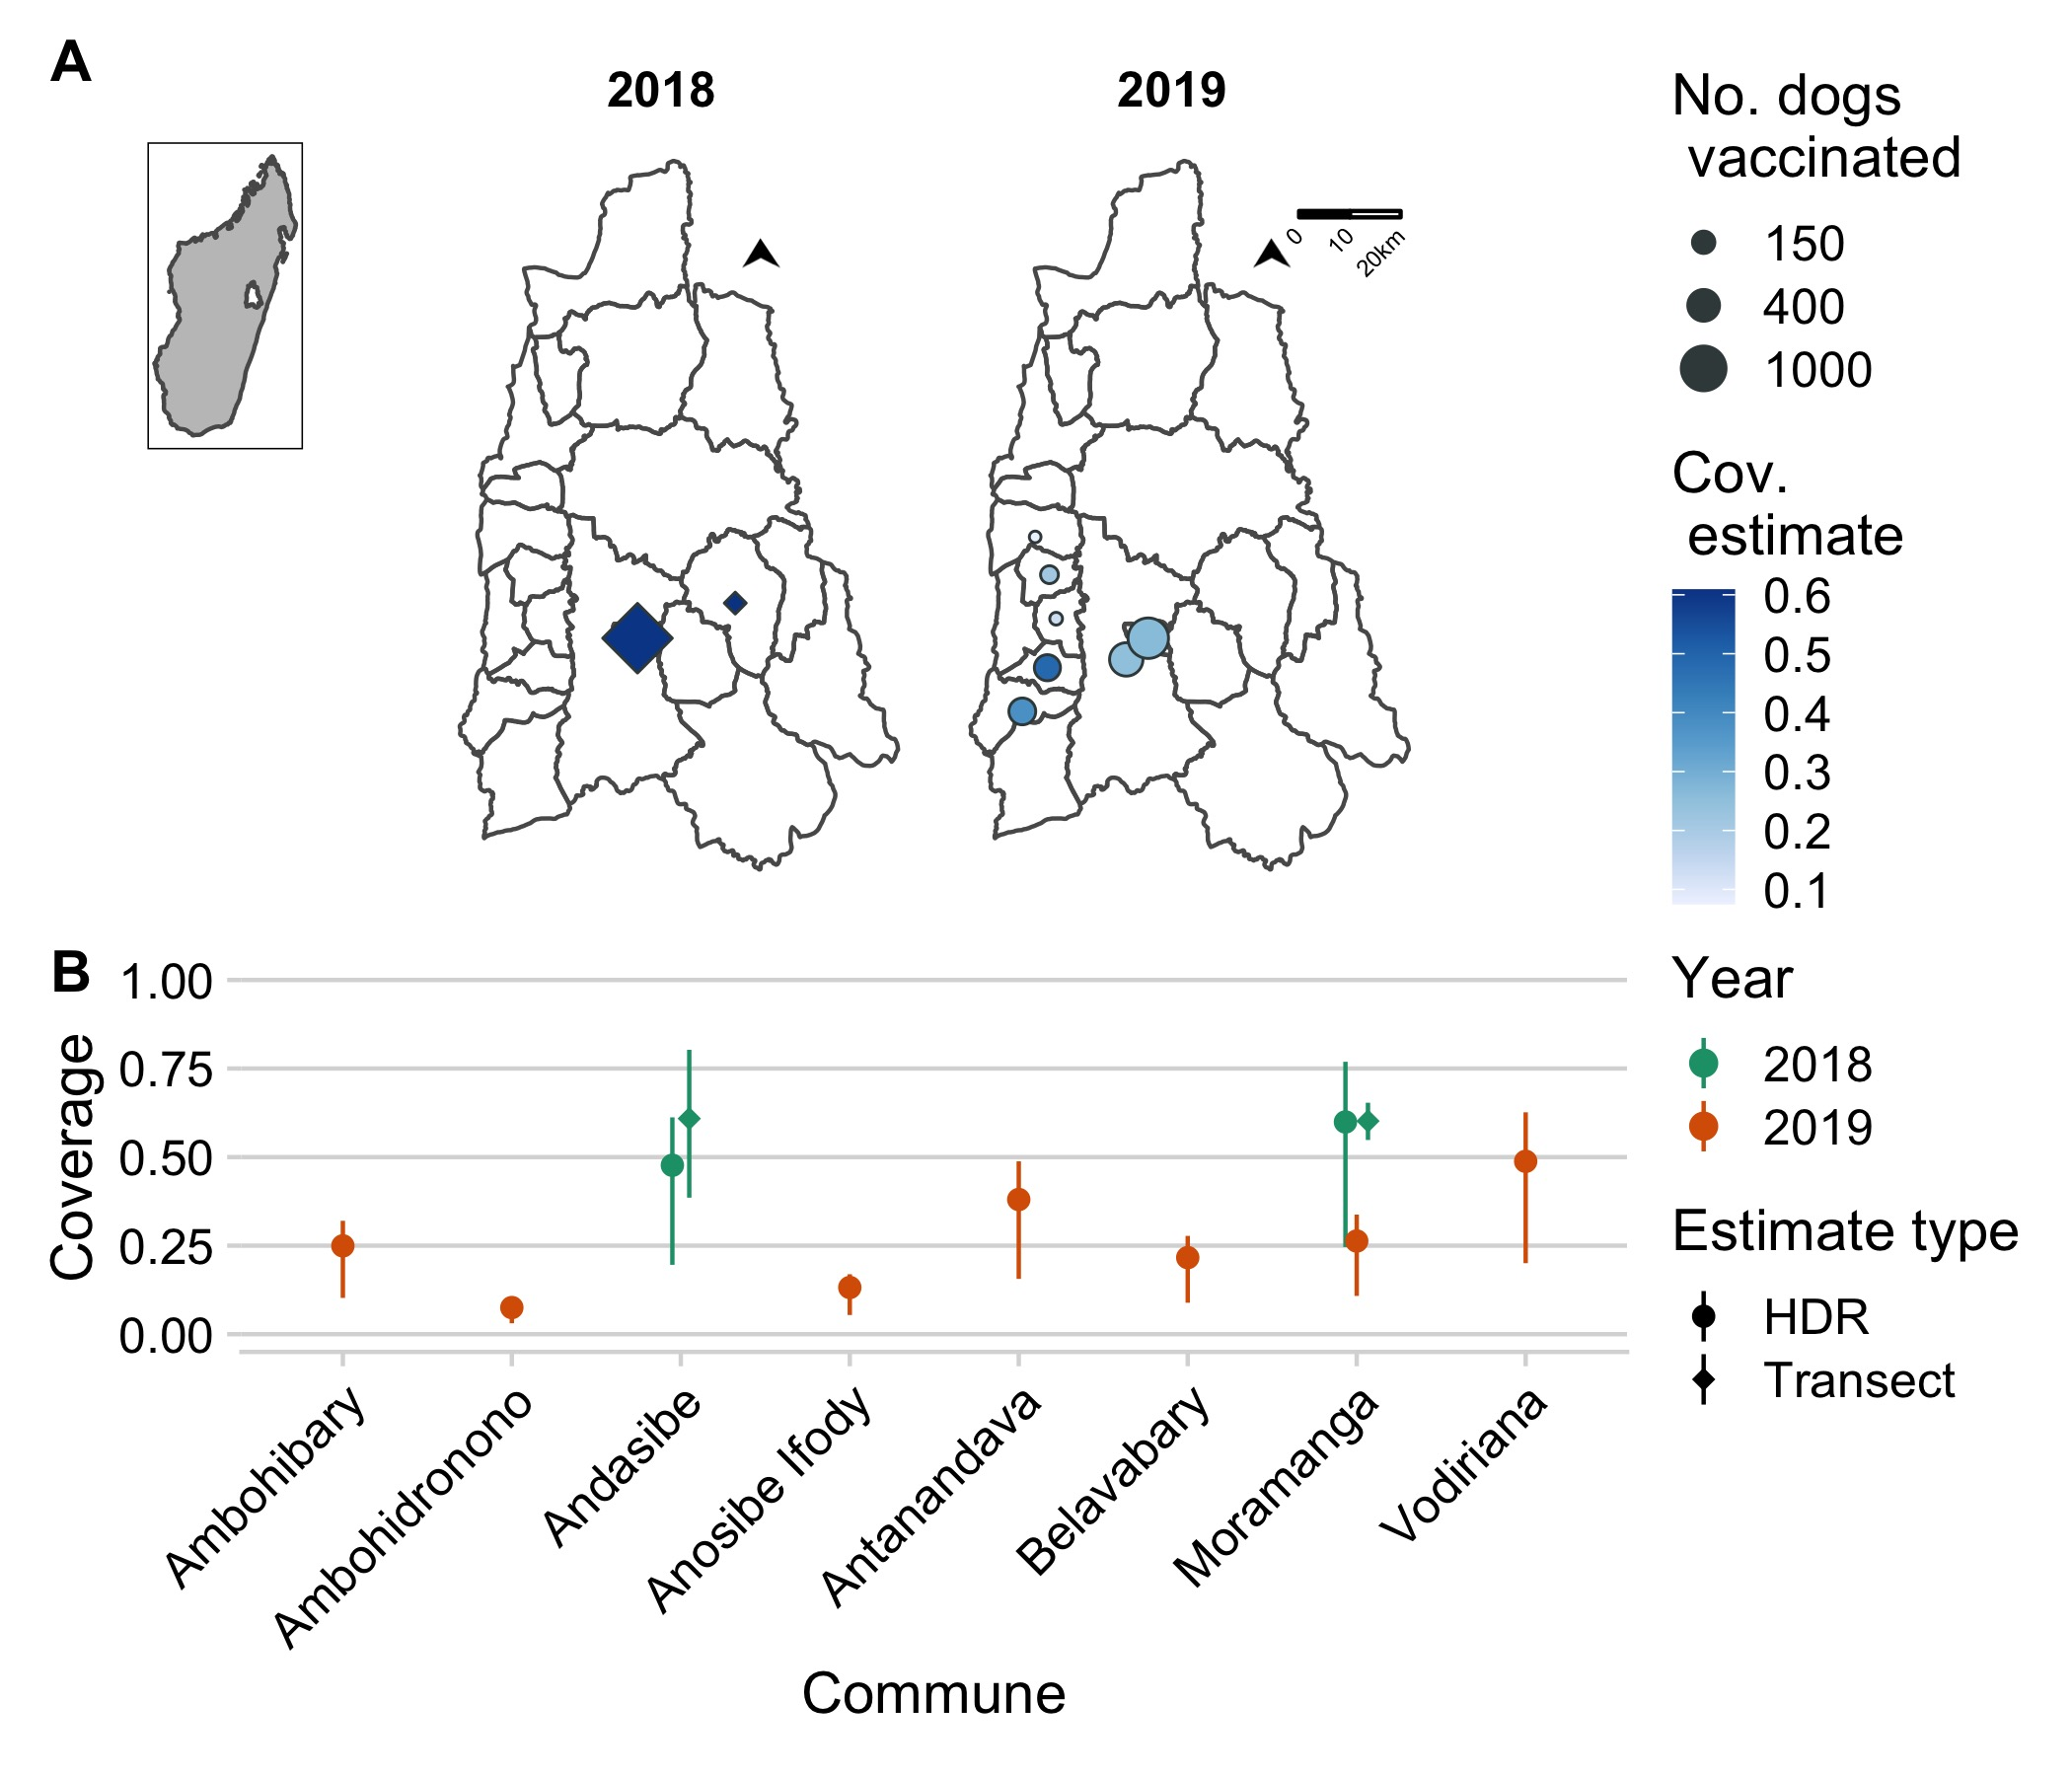
\includegraphics[width=0.8\linewidth]{/Users/mrajeev/Documents/Projects/mora_vax/figs/fig2}

\hypertarget{figure-2.-comparing-campaign-costs-and-willingness-to-pay.-a-vaccine-costs-broken-down-by-category-and-by-year-colors.-b-overall-cost-per-animal-vaccinated-for-the-two-campaign-years-split-by-direct-costs-of-vaccination-per-animal-i.e.-vaccine-vaccination-card-syringes-and-baseline-implementation-costs-i.e.-personnel-supplies-subsistence-costs-for-vaccinators-during-the-campaign.-c-estimated-cost-per-animal-vaccinated-under-a-willingness-to-pay-model-for-two-campaigns-examining-increasing-costs-charged-to-the-owner-with-estimated-costs-declining-due-to-cost-recovery-through-owner-payments-and-then-peaking-once-owners-report-to-be-no-longer-willing-to-pay-for-the-vaccine.-d-the-percent-reduction-in-number-of-animals-vaccinated-given-owners-willingness-to-pay.-the-curves-in-c-and-d-are-shown-based-on-the-overall-responses-on-willingness-to-pay-solid-line-from-both-moramanga-and-andasibe-and-the-responses-split-by-commune-dashed-and-dotted-lines.}{%
\paragraph{\texorpdfstring{\textbf{Figure 2. Comparing campaign costs
and willingness to pay}. \emph{A) Vaccine costs broken down by category
and by year (colors). B) Overall cost per animal vaccinated for the two
campaign years, split by direct costs of vaccination per animal
(i.e.~vaccine, vaccination card, syringes) and baseline implementation
costs (i.e.~personnel, supplies, subsistence costs for vaccinators
during the campaign). C) Estimated cost per animal vaccinated under a
willingness to pay model for two campaigns examining increasing costs
charged to the owner, with estimated costs declining due to cost
recovery through owner payments and then peaking once owners report to
be no longer willing to pay for the vaccine. D) The percent reduction in
number of animals vaccinated given owners willingness to pay. The curves
in C and D are shown based on the overall responses on willingness to
pay (solid line) from both Moramanga and Andasibe, and the responses
split by Commune (dashed and dotted
lines).}}{Figure 2. Comparing campaign costs and willingness to pay. A) Vaccine costs broken down by category and by year (colors). B) Overall cost per animal vaccinated for the two campaign years, split by direct costs of vaccination per animal (i.e.~vaccine, vaccination card, syringes) and baseline implementation costs (i.e.~personnel, supplies, subsistence costs for vaccinators during the campaign). C) Estimated cost per animal vaccinated under a willingness to pay model for two campaigns examining increasing costs charged to the owner, with estimated costs declining due to cost recovery through owner payments and then peaking once owners report to be no longer willing to pay for the vaccine. D) The percent reduction in number of animals vaccinated given owners willingness to pay. The curves in C and D are shown based on the overall responses on willingness to pay (solid line) from both Moramanga and Andasibe, and the responses split by Commune (dashed and dotted lines).}}\label{figure-2.-comparing-campaign-costs-and-willingness-to-pay.-a-vaccine-costs-broken-down-by-category-and-by-year-colors.-b-overall-cost-per-animal-vaccinated-for-the-two-campaign-years-split-by-direct-costs-of-vaccination-per-animal-i.e.-vaccine-vaccination-card-syringes-and-baseline-implementation-costs-i.e.-personnel-supplies-subsistence-costs-for-vaccinators-during-the-campaign.-c-estimated-cost-per-animal-vaccinated-under-a-willingness-to-pay-model-for-two-campaigns-examining-increasing-costs-charged-to-the-owner-with-estimated-costs-declining-due-to-cost-recovery-through-owner-payments-and-then-peaking-once-owners-report-to-be-no-longer-willing-to-pay-for-the-vaccine.-d-the-percent-reduction-in-number-of-animals-vaccinated-given-owners-willingness-to-pay.-the-curves-in-c-and-d-are-shown-based-on-the-overall-responses-on-willingness-to-pay-solid-line-from-both-moramanga-and-andasibe-and-the-responses-split-by-commune-dashed-and-dotted-lines.}}

\hypertarget{comparing-campaign-coverage-estimates}{%
\subsection{Comparing campaign coverage
estimates}\label{comparing-campaign-coverage-estimates}}

The 2018 campaign covered two communes and was estimated to have
achieved approximately 60\% coverage (fig 3A). The 2019 campaign covered
seven communes, but was estimated to have achieved lower coverage levels
(fig 3, ranging from 5 - 60\%). In the 2018 campaign, we used
post-vaccination coverage transects to estimate vaccination coverage,
but we were unable to do this in 2019 given the continuous delivery
strategy. In addition, in Andasibe in 2018, coverage estimates were
based on a single transect resulting in more uncertainty. However,
coverage estimates from the transects in 2018 were consistent with the
HDR based estimates (for both Andasibe and Moramanga, transect-based
estimates fell within the range of the HDR estimates). We also
back-calculated HDRs given our vaccination coverage estimates, and these
were similar to the HDRs calculated from the household survey (15.7 -
32.8 for Andasibe compared to 21.7 in a rural community and 17.8 - 21.2
for Moramanga Ville compared to 17.2 in an urban community).

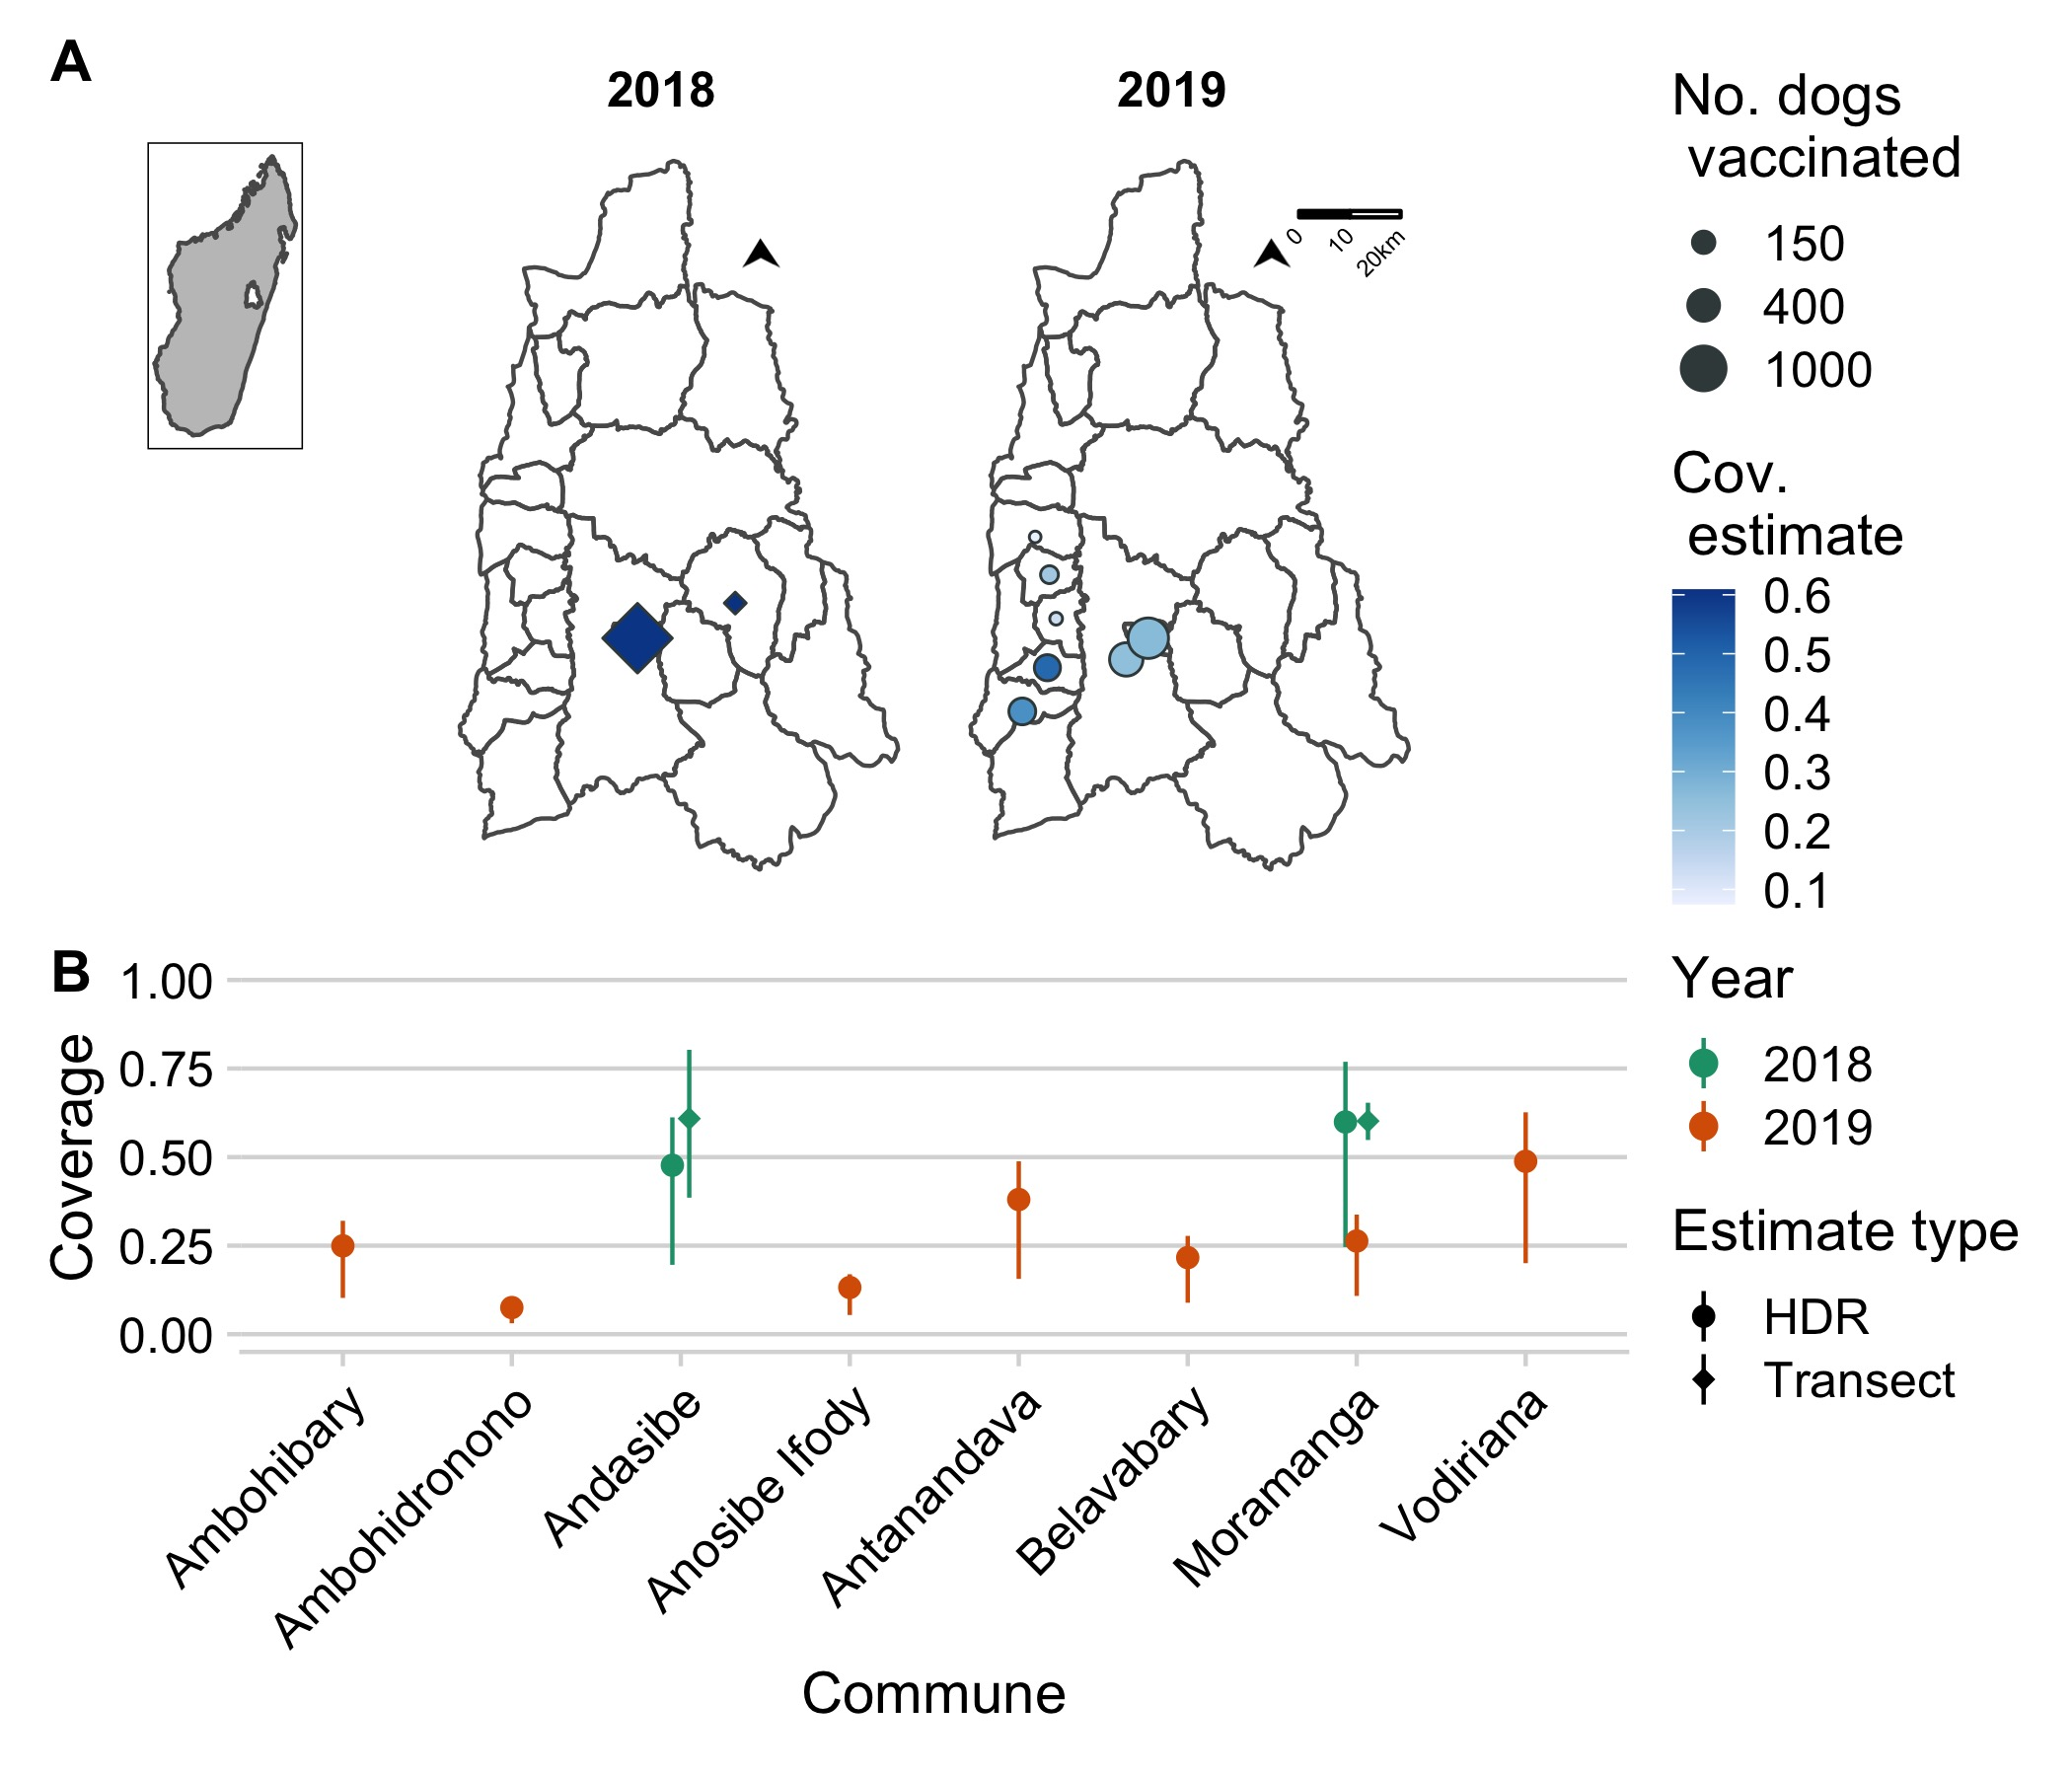
\includegraphics[width=0.8\linewidth]{/Users/mrajeev/Documents/Projects/mora_vax/figs/fig3}

\hypertarget{figure-3.-estimates-of-coverage-achieved-by-the-2018-and-2019-campaigns.-a-the-commune-level-numbers-of-dogs-vaccinated-size-of-points-and-the-associated-coverage-estimates-color-of-points-for-the-year-2018-estimated-using-post-vaccination-transects-and-2019-estimated-using-a-human-to-dog-ratio-hdr-of-19.5-based-on-a-recent-household-survey-in-the-moramanga-district.-the-inset-shows-the-location-of-the-moramanga-district-in-madagascar.-b-a-comparison-of-coverage-estimates-by-location-and-by-method-of-estimation-post-vaccination-transects-vs.-hdr-based-estimates-for-the-transect-based-estimates-the-line-range-shows-the-95-exact-binomial-confidence-interval-while-for-the-hdr-based-estimates-the-line-range-shows-the-range-of-coverage-estimates-assuming-an-hdr-range-of-8---25-according-to-estimates-from-the-literature.}{%
\paragraph{\texorpdfstring{\textbf{Figure 3. Estimates of coverage
achieved by the 2018 and 2019 campaigns}. \emph{A) The commune level
numbers of dogs vaccinated (size of points) and the associated coverage
estimates (color of points) for the year 2018 (estimated using
post-vaccination transects) and 2019 (estimated using a human-to-dog
ratio (HDR) of 19.5, based on a recent household survey in the Moramanga
District). The inset shows the location of the Moramanga District in
Madagascar. B) A comparison of coverage estimates by location and by
method of estimation (post-vaccination transects vs.~HDR based
estimates); for the transect based estimates, the line range shows the
95\% exact binomial confidence interval while for the HDR based
estimates, the line range shows the range of coverage estimates assuming
an HDR range of 8 - 25 according to estimates from the
literature.}}{Figure 3. Estimates of coverage achieved by the 2018 and 2019 campaigns. A) The commune level numbers of dogs vaccinated (size of points) and the associated coverage estimates (color of points) for the year 2018 (estimated using post-vaccination transects) and 2019 (estimated using a human-to-dog ratio (HDR) of 19.5, based on a recent household survey in the Moramanga District). The inset shows the location of the Moramanga District in Madagascar. B) A comparison of coverage estimates by location and by method of estimation (post-vaccination transects vs.~HDR based estimates); for the transect based estimates, the line range shows the 95\% exact binomial confidence interval while for the HDR based estimates, the line range shows the range of coverage estimates assuming an HDR range of 8 - 25 according to estimates from the literature.}}\label{figure-3.-estimates-of-coverage-achieved-by-the-2018-and-2019-campaigns.-a-the-commune-level-numbers-of-dogs-vaccinated-size-of-points-and-the-associated-coverage-estimates-color-of-points-for-the-year-2018-estimated-using-post-vaccination-transects-and-2019-estimated-using-a-human-to-dog-ratio-hdr-of-19.5-based-on-a-recent-household-survey-in-the-moramanga-district.-the-inset-shows-the-location-of-the-moramanga-district-in-madagascar.-b-a-comparison-of-coverage-estimates-by-location-and-by-method-of-estimation-post-vaccination-transects-vs.-hdr-based-estimates-for-the-transect-based-estimates-the-line-range-shows-the-95-exact-binomial-confidence-interval-while-for-the-hdr-based-estimates-the-line-range-shows-the-range-of-coverage-estimates-assuming-an-hdr-range-of-8---25-according-to-estimates-from-the-literature.}}

\hypertarget{dog-demography-and-simulating-vaccination-strategies}{%
\subsection{Dog demography and simulating vaccination
strategies}\label{dog-demography-and-simulating-vaccination-strategies}}

Demographic data from vaccinated dogs shows a population pyramid with a
large base, indicative of a fast-growing population, and with a male
bias (approximately 60\% male, Fig 4A). We fit these data to an
age-structured model, and were able to generate parameter estimates
which resulted in stable age distributions consistent with the data (Fig
4B). We filter to parameter estimates that are consistent with a growing
population resulting in mean adult annual survival probability of 0.77
(95\% quantile: 0.59 - 0.97). We use estimates of fertility (on average
1.09, 95\% quantile: 0.82 - 1.41) to back-calculate pup survival, which
ranges from 0.34 - 0.68. We find that given these demographic
parameters, annual campaigns that target dogs of all ages result in
rapid decline in vaccination coverage between campaigns, largely due to
rapid turnover of the dog population (compared to the impact of waning
immunity assuming a discrete 3 year period of vaccine immunity, evident
in the additional dip at year 3, fig 4D). Continuously targeting 70\% of
the puppy population for vaccination, while unable to achieve the peak
coverage, consistently reaches coverage of about 50\% of the dog
population. A combined strategy maintains the highest and most
temporally stable levels of coverage close to the target of 70\%.

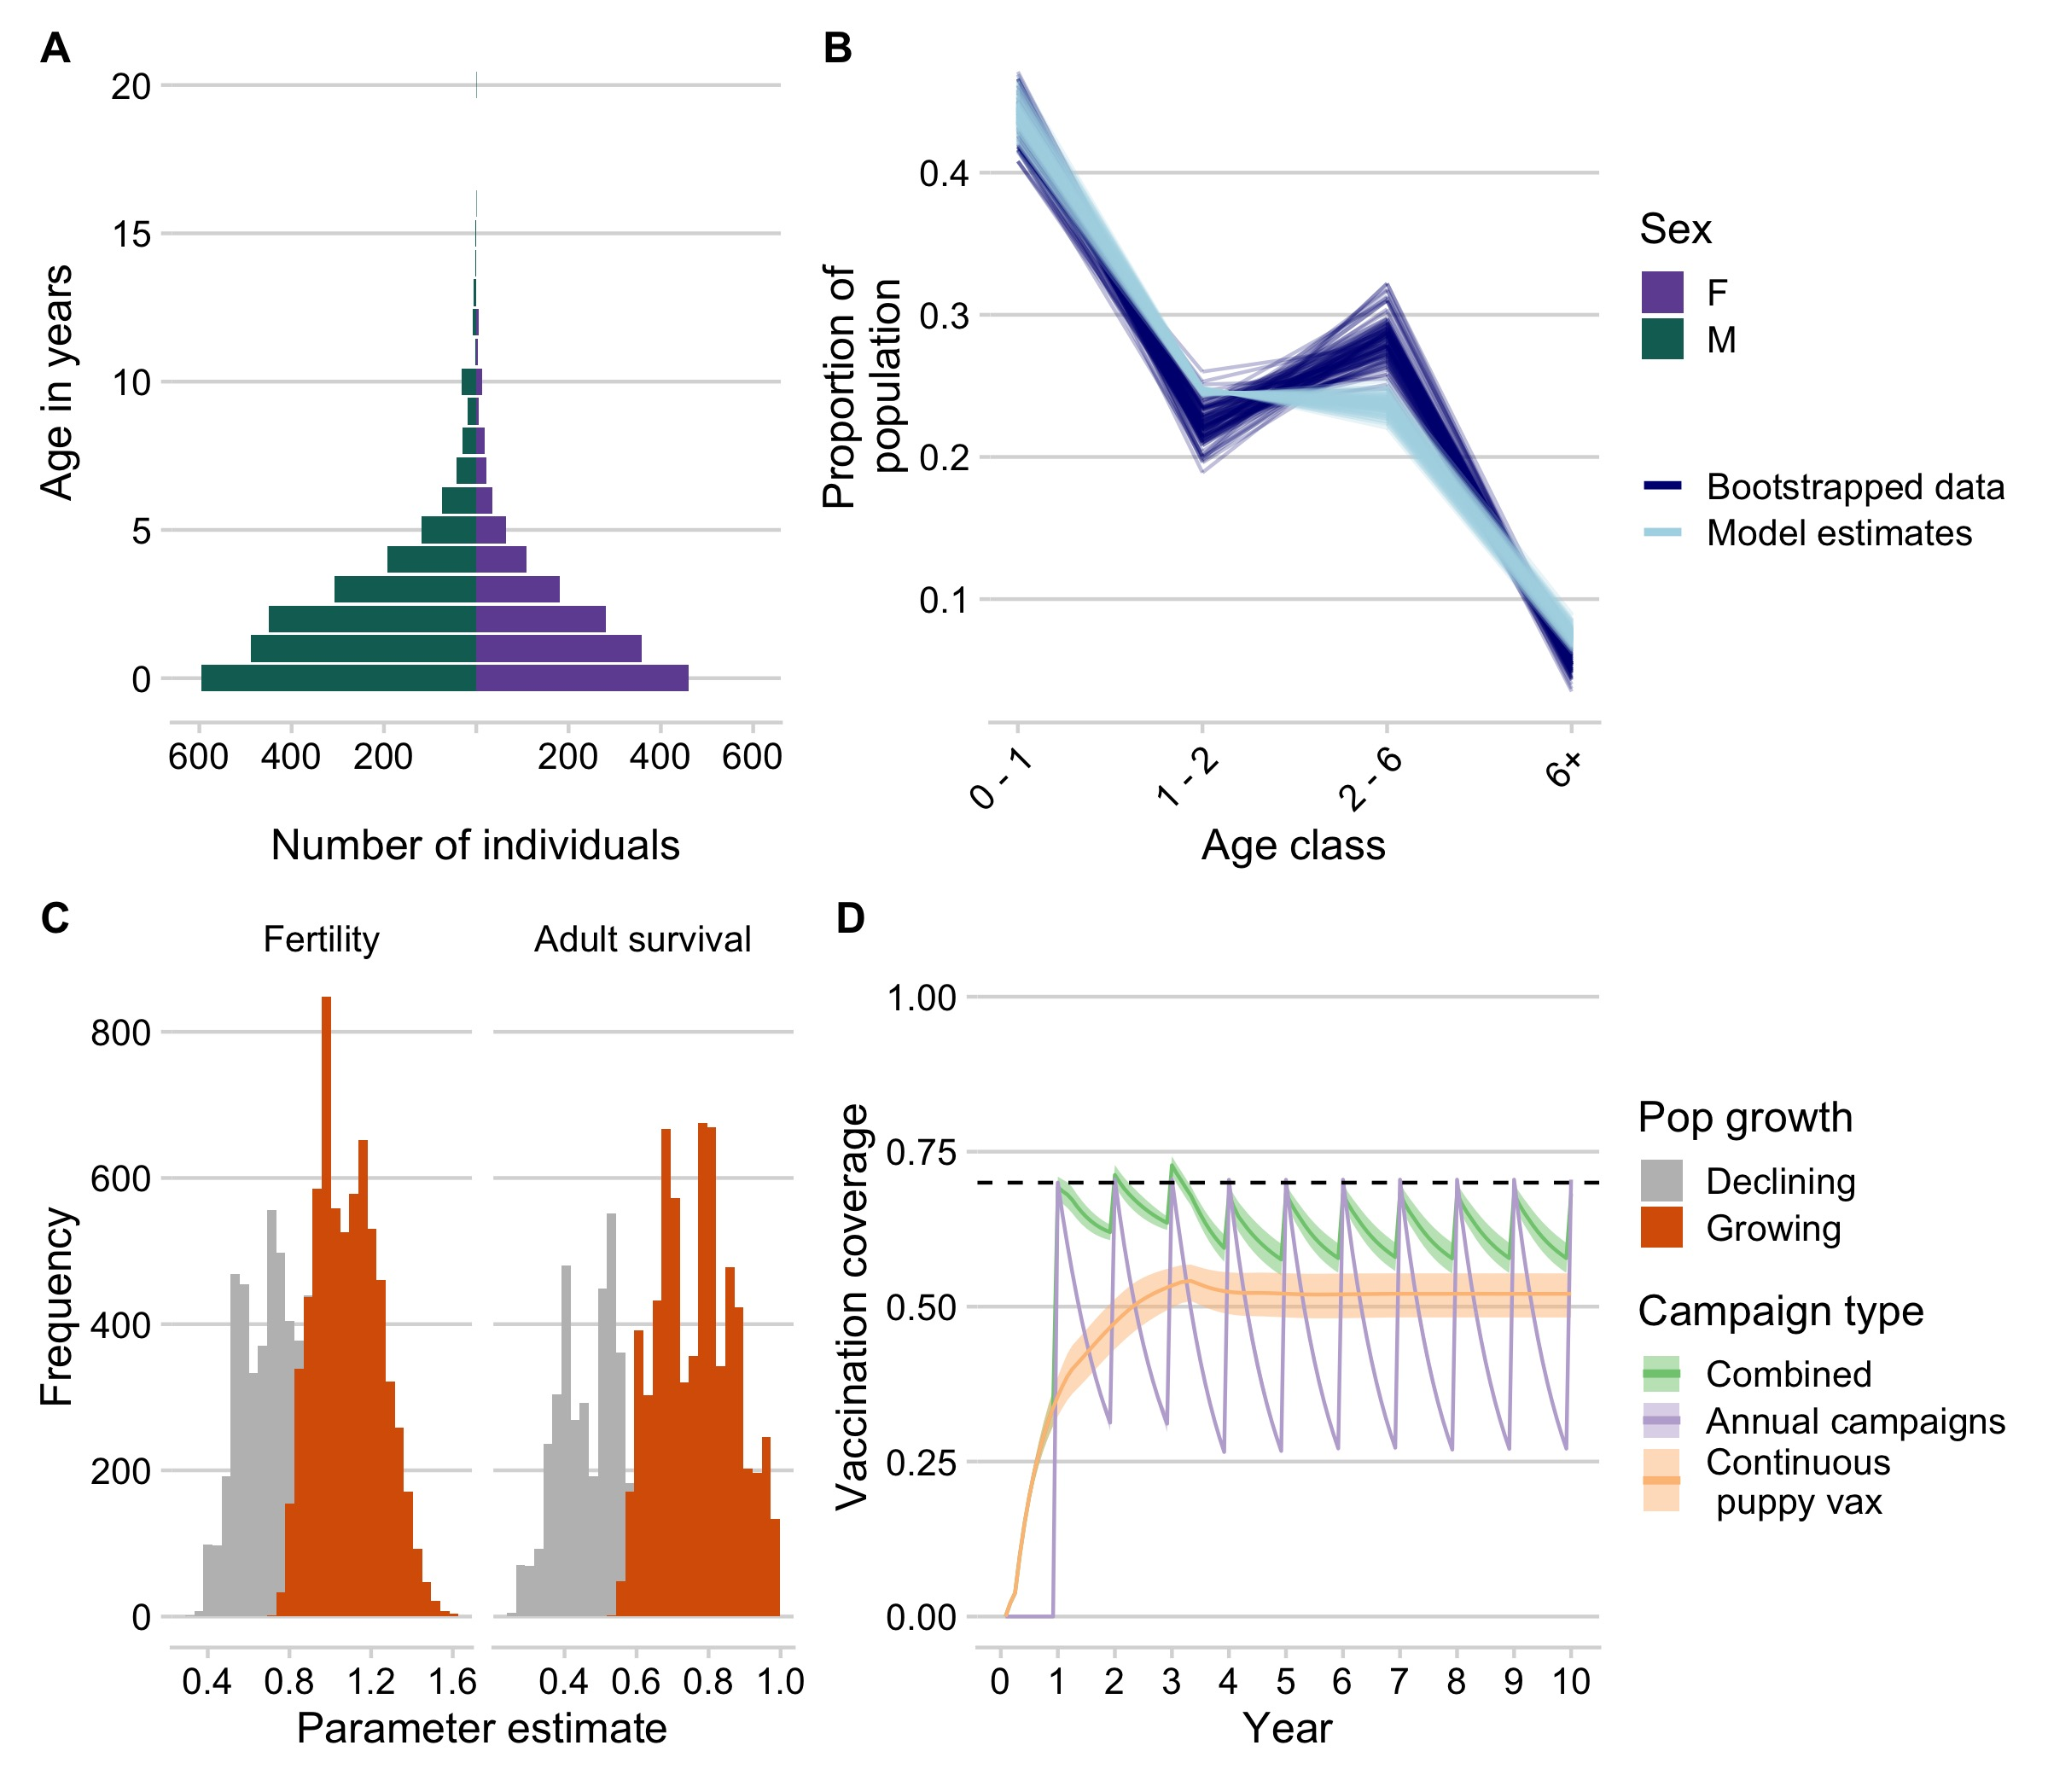
\includegraphics[width=0.8\linewidth]{/Users/mrajeev/Documents/Projects/mora_vax/figs/fig4}

\hypertarget{figure-4.-dog-demography-and-implications-for-campaign-strategies.-a-the-age-pyramid-for-vaccinated-dogs-by-sex.-b-bootstrapped-estimates-of-the-proportion-of-the-population-in-each-age-class-from-the-age-data-dark-blue-compared-to-estimates-from-the-demographic-models-fit-to-these-data-light-blue.-c-parameter-estimates-for-annual-fertility-rates-and-adult-survival-probability-with-estimates-highlighted-in-orange-showing-the-parameter-estimates-which-result-in-positive-population-growth.-b-simulated-vaccination-coverage-n-1000-using-the-demographic-parameters-from-c-in-a-hypothetical-commune-with-1000-dogs-for-three-different-campaign-strategies-1-annual-vaccination-campaigns-targeting-dogs-of-all-ages-purple-2-routine-vaccination-of-puppies-at-3-months-of-age-and-3-a-combined-strategy-with-campaigns-annually-and-continuous-puppy-vaccination-in-between-campaigns.}{%
\paragraph{\texorpdfstring{\textbf{Figure 4. Dog demography and
implications for campaign strategies}. \emph{A) The age pyramid for
vaccinated dogs by sex. B) Bootstrapped estimates of the proportion of
the population in each age class from the age data (dark blue) compared
to estimates from the demographic models fit to these data (light blue).
C) Parameter estimates for annual fertility rates and adult survival
probability, with estimates highlighted in orange showing the parameter
estimates which result in positive population growth. B) Simulated
vaccination coverage (N = 1000) using the demographic parameters from
(C) in a hypothetical commune with 1000 dogs for three different
campaign strategies: 1) annual vaccination campaigns targeting dogs of
all ages (purple), 2) routine vaccination of puppies at 3 months of age,
and 3) a combined strategy with campaigns annually and continuous puppy
vaccination in between
campaigns.}}{Figure 4. Dog demography and implications for campaign strategies. A) The age pyramid for vaccinated dogs by sex. B) Bootstrapped estimates of the proportion of the population in each age class from the age data (dark blue) compared to estimates from the demographic models fit to these data (light blue). C) Parameter estimates for annual fertility rates and adult survival probability, with estimates highlighted in orange showing the parameter estimates which result in positive population growth. B) Simulated vaccination coverage (N = 1000) using the demographic parameters from (C) in a hypothetical commune with 1000 dogs for three different campaign strategies: 1) annual vaccination campaigns targeting dogs of all ages (purple), 2) routine vaccination of puppies at 3 months of age, and 3) a combined strategy with campaigns annually and continuous puppy vaccination in between campaigns.}}\label{figure-4.-dog-demography-and-implications-for-campaign-strategies.-a-the-age-pyramid-for-vaccinated-dogs-by-sex.-b-bootstrapped-estimates-of-the-proportion-of-the-population-in-each-age-class-from-the-age-data-dark-blue-compared-to-estimates-from-the-demographic-models-fit-to-these-data-light-blue.-c-parameter-estimates-for-annual-fertility-rates-and-adult-survival-probability-with-estimates-highlighted-in-orange-showing-the-parameter-estimates-which-result-in-positive-population-growth.-b-simulated-vaccination-coverage-n-1000-using-the-demographic-parameters-from-c-in-a-hypothetical-commune-with-1000-dogs-for-three-different-campaign-strategies-1-annual-vaccination-campaigns-targeting-dogs-of-all-ages-purple-2-routine-vaccination-of-puppies-at-3-months-of-age-and-3-a-combined-strategy-with-campaigns-annually-and-continuous-puppy-vaccination-in-between-campaigns.}}

\hypertarget{discussion}{%
\section{Discussion}\label{discussion}}

Through vaccination campaigns implemented in Moramanga District of
Madagascar, we saw high demand for vaccination from dog owners and found
that dogs were accessible and able to be handled safely and efficiently
for parenteral vaccination at a reasonable cost (between 1.3 - 1.8 USD
per animal vaccinated). We find that providing the vaccine at no direct
cost to dog owners will be critical to achieving sufficient coverage, as
even with nominal fees, a significant proportion of owners indicated
they would no longer vaccinate their animals. A static point vaccination
strategy achieved higher coverage over a shorter time period in 2018
compared to dog vaccinations conducted by the District Veterinarian as
part of routine veterinary service provision in 2019. However, it came
at a higher cost per animal vaccinated, was more limited in geographic
scope, and required more resources in terms of personnel. In addition,
in the rural setting of Andasibe, the static point campaign strategy
achieved lower coverage, reflecting less accessible, hard-to-reach human
communities in this location. Based on the lessons learned through these
campaigns, in particular the observation that puppies were relatively
easy to handle for vaccinators and owners, we find that continuous
vaccination targeting puppies in particular may be an effective way to
maintain vaccination coverage levels given high turnover in dog
populations.

There were several limitations to our analyses. Owner reports of
willingness to pay, age of animals, and distance travelled to the
vaccination point likely all suffer from recall bias and uncertainty,
whilst willingness to pay studies are often overestimates of observed
practice \citep{birhane2016}. In addition, the age of animals brought to
vaccination points may not be representative of the age structure of the
underlying population, and other work has shown that in general puppies
(individuals \textless{} 1 year) tend to have lower vaccination coverage
than adults
\citep{arief2016, sanchez-soriano2020, mazeri2019, minyoo2015}.
Additionally, we did not vaccinate animals less than 1 month of age,
which may explain why we sometimes estimated declining populations (as
part of the age class of 0-1 years was not captured by the data).
However, our analyses based on these data are consistent with previous
findings from SSA that demonstrate male-biased populations, skewed
towards puppies, and with high mortality in the first year of life
\citep{czupryna2016, taylor2017}. Studies have also shown that charging
fees for vaccines can greatly reduce the efficacy of campaigns and are a
significant barrier to vaccination for owners
\citep{schildecker2016, yoak2021, barbosacosta2020}. Similarly, distance
to campaign points has been identified as a barrier to vaccination, and
in most cases owners report traveling less than 1km to reach a
vaccination point \citep{mazeri2018barriers, mazeri2019}. We used HDRs,
which can be sensitive to underlying estimates of the human population
and the spatial scale of estimation
\citep{sambo2018estimating, sambo2017}. However, we used HDR estimates
from a recent household survey study in the district, and found these to
give coverage estimates consistent with those from post-vaccination
transects. Finally, in our vaccination model, we make several
simplifying assumptions: we assume that immunity wanes after three years
(simulating vaccination with a long-lasting vaccine such as Nobivac),
but we also assume that vaccinated dogs that survive to the following
year are revaccinated in subsequent campaigns (effectively assuming
boosting per manufacturer recommendations for Rabisin). Overall waning
vaccinal immunity plays a lesser role in declining vaccination coverage
given the high population turnover in this context. In our
age-structured models, we also do not account for population carrying
capacity, which likely overestimates growth of the dog population.

Our estimates of costs per animal vaccinated are in line with recent
estimates from other countries \citep{undurraga2020}, although we likely
underestimate costs given the donation of time and resources by the
organizations and individuals involved (i.e.~costs associated with
international volunteers including airfare and visa costs as well as
costs of transportation donated to the campaign). We also did not
include costs of pre-exposure prophylaxis as all of our volunteers and
vaccinators had been vaccinated prior to the campaigns. Both pre- and
post-exposure vaccines should however always be readily available for
vaccinators and should be included in vaccination program budgets. While
the volunteer-led effort resulted in significant financial and personnel
resources being devoted to the campaign, costs were higher overall and
per animal vaccinated. In addition, NGO and volunteer based campaigns
may be difficult to sustain given unpredictable funding, time
commitments, and turnover in staff \citep{ferguson2020}. Dog vaccination
delivered through the District Veterinarian was less costly, with the
majority of the costs directly related to vaccination. Although we
included costs of implementing transect based coverage estimates, these
were negligible (less than 0.10 USD per dog vaccinated), in line with
recent studies which have shown this strategy is a cheap and effective
way to estimate coverage \citet{sambo2017}; \citet{gibson2015}{]}.

One key aspect we do not consider is potential feedback loops between
vaccination and demography. Estimates of the effects of vaccination on
dog demography are mixed \citep{czupryna2016}, but vaccination may
increase dog survival \citep{conan2015}. If dog population growth is
driven by survival, then this could mean that increased vaccination
results in increased population growth. However, if growth is driven
more by demand from human communities, then vaccination could stabilize
the population and reduce population turnover. Improving dog population
management, encouraging responsible pet ownership practices, and
increasing veterinary services could all complement vaccination efforts,
but have not been demonstrated to result in meaningful rabies control
without parallel dog vaccination \citep{taylor2017}.

In settings with high dog ownership, moving towards community-based
vaccination strategies could be an effective way to achieve sufficient
and consistent coverage, particularly in hard-to-reach communities.
During our campaign, we found that puppies at approximately 3 months old
were easy to handle for both vaccinators and owners. Puppy vaccination
could be carried out by local officials embedded in communities (along
the lines of community health workers), especially given recent findings
on thermotolerance of rabies vaccines and locally manufactured methods
for maintaining temperatures required for sustained vaccine storage (up
to 3 months) \citep{lugelo2020}. Incentivizing vaccinators appropriately
will be a key challenge, as currently providing no-cost rabies
vaccination is not seen as part of routine duties for district
veterinarians or for livestock officers. Implementing dog vaccination
alongside government mandated livestock vaccination campaigns may also
be a strategy to scale up vaccination efforts at relatively low-cost.
Expanding veterinary services across the country and relieving financial
pressures on veterinarians and animal health workers through appropriate
compensation could greatly improve veterinary services across Madagascar
\citep{mondiale2017evaluation}. For volunteer based efforts, focusing on
local volunteers (i.e.~veterinary students) may be a more cost-effective
strategy. However similar to international volunteers, volunteers
require subsistence during vaccination campaigns when not based in the
communities where they study or live.

Overall, our results suggest that dog vaccination is a feasible and
effective strategy for controlling canine rabies in Madagascar. However,
rabies vaccination must be recognized as a public good. Strategies to
remove barriers for dog owners and to incentivize veterinarians and
other animal health workers to implement vaccination will be key to
long-term campaign success. Borrowing strategies from human vaccination
efforts, i.e.~deploying community health workers, could be a way to
deliver vaccinations and reduce costs in the hardest-to-reach
communities. In addition, refining vaccination strategies to local
contexts and using improved tools and systems, such as mobile phone
based data collection, could improve efficacy and lower costs of
campaigns \citep{mazeri2021, gibson2016a}. To monitor the success of
these campaigns, it will be critical to develop efficient and effective
methods to estimate vaccination coverage and to measure their impact on
reducing rabies incidence through robust surveillance
\citep{lushasi2020, ferguson2020}. With limited chances for
reintroduction from outside the island, Madagascar could be a model for
rabies elimination, and strategies that tackle the context specific
challenges could be a path forward for the country to reach ZeroBy30.

% %%%%%%%%%%%%%%%%%%%%%%%%%%%%%%%%%%%%%%%%%%
% %% optional
% \supplementary{The following are available online at www.mdpi.com/link, Figure S1: title, Table S1: title, Video S1: title.}
%
% % Only for the journal Methods and Protocols:
% % If you wish to submit a video article, please do so with any other supplementary material.
% % \supplementary{The following are available at www.mdpi.com/link: Figure S1: title, Table S1: title, Video S1: title. A supporting video article is available at doi: link.}

\vspace{6pt}

%%%%%%%%%%%%%%%%%%%%%%%%%%%%%%%%%%%%%%%%%%
\acknowledgments{We thank all the veterinarians, livestock officers,
local officials and leaders, NGO staff, and volunteers involved in each
of the campaigns. We are grateful to staff and officials at the
Department of Veterinary Services, the Ministry of Public Health, and
the Institut Pasteur de Madagascar for their support and technical
assistance. In particular, we thank Carmen Barba Claassens, Jean
Hyacinthe Randrianarisoa, Ranaivoarimanana, Fierenantsoa
Randriamahatana, Esther Noiarisaona, Cara Brook, and Christian
Ranaivoson, Rila Ratovoson, and Claire LeBlanc. The campaign costs were
supported by donations from Lush Cosmetics Charity Pot. Parts of this
work were funded by grants from the Center for Health and Wellbeing and
the Department of Ecology and Evolutionary Biology at Princeton
University to MR. MR was supported by an NSF Graduate Research
Fellowship and a Princeton Institute for Regional and International
Studies Graduate Fellowship. KH is supported by the Wellcome Trust
(207569/Z/17/Z). We want to particularly acknowledge the contributions
to this work by Annie Yang, an undergraduate researcher and volunteer
with Princeton University and the Mad Dog Initiative who tragically
passed away in a car accident before this research was published.}

%%%%%%%%%%%%%%%%%%%%%%%%%%%%%%%%%%%%%%%%%%

%%%%%%%%%%%%%%%%%%%%%%%%%%%%%%%%%%%%%%%%%%
\conflictsofinterest{The authors declare no conflict of interest. The
funders had no role in the design of the study; in the collection,
analyses, or interpretation of data; in the writing of the manuscript,
or in the decision to publish the results.}

%%%%%%%%%%%%%%%%%%%%%%%%%%%%%%%%%%%%%%%%%%
%% optional


%%%%%%%%%%%%%%%%%%%%%%%%%%%%%%%%%%%%%%%%%%
% Citations and References in Supplementary files are permitted provided that they also appear in the reference list here.

%=====================================
% References, variant A: internal bibliography
%=====================================
%\reftitle{References}
%\begin{thebibliography}{999}
% Reference 1
%\bibitem[Author1(year)]{ref-journal}
%Author1, T. The title of the cited article. {\em Journal Abbreviation} {\bf 2008}, {\em 10}, 142--149.
% Reference 2
%\bibitem[Author2(year)]{ref-book}
%Author2, L. The title of the cited contribution. In {\em The Book Title}; Editor1, F., Editor2, A., Eds.; Publishing House: City, Country, 2007; pp. 32--58.
%\end{thebibliography}

% The following MDPI journals use author-date citation: Arts, Econometrics, Economies, Genealogy, Humanities, IJFS, JRFM, Laws, Religions, Risks, Social Sciences. For those journals, please follow the formatting guidelines on http://www.mdpi.com/authors/references
% To cite two works by the same author: \citeauthor{ref-journal-1a} (\citeyear{ref-journal-1a}, \citeyear{ref-journal-1b}). This produces: Whittaker (1967, 1975)
% To cite two works by the same author with specific pages: \citeauthor{ref-journal-3a} (\citeyear{ref-journal-3a}, p. 328; \citeyear{ref-journal-3b}, p.475). This produces: Wong (1999, p. 328; 2000, p. 475)

%=====================================
% References, variant B: external bibliography
%=====================================
\reftitle{References}
\externalbibliography{yes}
\bibliography{mybibfile.bib}

%%%%%%%%%%%%%%%%%%%%%%%%%%%%%%%%%%%%%%%%%%
%% optional

%% for journal Sci
%\reviewreports{\\
%Reviewer 1 comments and authors’ response\\
%Reviewer 2 comments and authors’ response\\
%Reviewer 3 comments and authors’ response
%}

%%%%%%%%%%%%%%%%%%%%%%%%%%%%%%%%%%%%%%%%%%
\end{document}
